\documentclass{article}
\usepackage{arxiv}

\usepackage[utf8]{inputenc}
\usepackage[english, russian]{babel}
\usepackage[T1]{fontenc}
\usepackage{url}
\usepackage{booktabs}
\usepackage{amsfonts}
\usepackage{nicefrac}
\usepackage{microtype}
\usepackage{lipsum}
\usepackage{graphicx}
\usepackage{natbib}
\usepackage{doi}



\title{Адаптация методов обучения с подкреплением в задаче обучения LLM}

\author{\textbf{Денисов Егор Александрович} \\
	МГУ им. М.В.Ломоносова \\
	Факультет ВМК, кафедра ММП\\
	Москва, Россия \\
	\texttt{s02220081@gse.cs.msu.ru} \\
	%% examples of more authors
	\And
	\textbf{Сердюк Юлиан Анатольевич} \\
	МГУ им. М.В.Ломоносова \\
	Факультет ВМК, кафедра ММП \\
	Москва, Россия \\
	% \texttt{stariate@ee.mount-sheikh.edu} \\
	%% \AND
	%% Coauthor \\
	%% Affiliation \\
	%% Address \\
	%% \texttt{email} \\
	%% \And
	%% Coauthor \\
	%% Affiliation \\
	%% Address \\
	%% \texttt{email} \\
	%% \And
	%% Coauthor \\
	%% Affiliation \\
	%% Address \\
	%% \texttt{email} \\
}
\date{}

\renewcommand{\shorttitle}{\textit{arXiv} Template}

%%% Add PDF metadata to help others organize their library
%%% Once the PDF is generated, you can check the metadata with
%%% $ pdfinfo template.pdf
\hypersetup{
pdftitle={A template for the arxiv style},
pdfsubject={q-bio.NC, q-bio.QM},
pdfauthor={David S.~Hippocampus, Elias D.~Striatum},
pdfkeywords={First keyword, Second keyword, More},
}

\begin{document}
\maketitle

\begin{abstract}
	Современные большие языковые модели (БЯМ) демонстрируют впечатляющие способности к рассуждению, обобщению и генерации текста, однако их эффективность во многом зависит от качества этапов дообучения — дообучения с учителем (англ. SFT) и обучения с подкреплением (англ. RL). Несмотря на то, что данные подходы обширно изучаются, остаются открытыми вопросы о том, как корректно их совмещать для достижения наилучшего качества. В данной работе рассматриваются подходы к адаптации методов обучения с подкреплением для задач дообучения БЯМ с особым вниманием к двум аспектам - комбинации функции потерь и оптимальному чередованию этапов обучения. Эксперименты выполняются на стандартных бенчмарках для тестирования математического и логического рассуждения модели. Анализ результатов показывает, что гибридные схемы, предложенные нами, обеспечивают лучшее соотношение между устойчивостью, скоростью сходимости и способностью к обобщению.
\end{abstract}


% \keywords{First keyword \and Second keyword \and More}

\section{Introduction}
Современные большие языковые модели (БЯМ) становятся основным инструментом в задачах обработки естественного языка и генерации текста. Однако для достижения высокой точности и способности к обобщению им необходимо сложное многоэтапное обучение, включающее в себя различные этапы. Актуальность исследований в этой области обусловлена необходимостью повышения устойчивости, управляемости и эффективности БЯМ при решении задач, требующих рассуждений и логических выводов.

На сегодняшний день одним из ключевых направлений развития БЯМ является совершенствование этапов дообучения, в частности SFT и RL. Основной подход на стадии RL - обучение с подкреплением на основе человеческих ответов (англ. RLHF), а также различные его улучшения. В качестве последних выступают различные модификации функции вознаграждения, стратегий обновления модели и схем совмещения RL с традиционным SFT.

Тем не менее, существующие решения имеют ряд ограничений. Во-первых, большинство подходов не учитывают сложное взаимодействие между этапами SFT и RL, что может приводить к забыванию уже приобретённых моделью знаний. Во-вторых, функции вознаграждения зачастую плохо коррелируют с реальными показателями качества текста, особенно в задачах рассуждения. В-третьих, в RLHF используются данные собранные в онлайн-режиме. Зачастую такие данные ограничены, и используемые методы оптимизации нередко страдают от нестабильности и переобучения.

В данной работе предлагается подход к адаптации методов обучения с подкреплением для дообучения БЯМ, основанный на гибридной схеме чередования этапов SFT и RL с комбинированной функцией потерь. Такой подход позволяет учитывать как сигналы от данных с учителем, так и награды, поступающие из среды. Особое внимание уделяется исследованию стратегий управления частотой переходов между режимами обучения и влиянию этих переходов на стабильность оптимизации. Кроме того, рассматриваются модификации функции вознаграждения, направленные на повышение чувствительности к ошибкам логического вывода.

Модели, обученные с использованием предложенного подхода, демонстрируют более быструю сходимость и лучшую способность к обобщению по сравнению с классическим RLHF. Таким образом, представленные результаты вносят вклад в развитие методологий дообучения БЯМ, предлагая более гибкий и устойчивый механизм совмещения SFT и RL, что открывает новые перспективы для дальнейшего повышения качества языковых моделей.


\section{Related works}
\subsection{Парадигмы обучения}
Дообучение с учителем является основополагающей техникой для адаптации больших языковых моделей под специфичные задачи. Благодаря своей эффективности, данный подход стал широко применим в различных областях, в том числе и в решении математических задач (Cobbe et al. 2021a; Hendrycks et al. 2021; Yuan et al. 2023). Тем не менее, чистый SFT позволяет хорошо выучить шаблоны решений, но не помогает улучшить способность модели к рассуждению. Причиной этому служат ограниченные и несбалансированные данные, неоптимальная для данной задачи функция потерь.

Для решения существующих проблем после стадии SFT стало применяться обучение с подкреплением. Таким образом, SFT позволяет достичь высокого базового качества, а RL улучшает эффективность и подстраивает поведение модели под конкретную задачу. Ярким примером совмещения двух парадигм является \texttt{DeepSeekMath} (Shao et al. 2024)

\subsection{Совмещение SFT и RL}
Последовательное выполнение стадий SFT и RL также имеет свои ограничения и недостатки. Вследствие этого исследуются способы динамически совмещать данные подходы. Так, в работах Ma et al. 2025, Liu et al. 2025 предлагаются схожие стратегии чередования RL и SFT, где RL служит основой обучения, а SFT применяется для наиболее сложных примеров в выборке.

Другой класс работ предлагает пошаговую адаптацию и мониторинг тренировочной динамики: SASR (Chen et al. 2025) и близкие методы отслеживают градиентные нормы и распределение выходов модели, чтобы динамически корректировать вклад SFT и RL на каждом шаге обучения и тем самым уменьшить эффект катастрофического забывания и переобучения.

Наконец, в сторону более формализованных схем кооперации шагнул BRIDGE (Chen et al. 2025), который использует двухуровневую оптимизацию для одновременного обучения «нижнего» уровня (RL-обновления) и «верхнего» уровня (SFT). Такая кооперативная постановка направлена на то, чтобы SFT на каждой итерации предоставлял улучшенную инициализацию для стадии обучения с подкреплением, что даёт прирост итоговой точности.



\section{Headings: first level}
\label{sec:headings}

\lipsum[4] See Section \ref{sec:headings}.

\subsection{Headings: second level}
\lipsum[5]
\begin{equation}
	\xi _{ij}(t)=P(x_{t}=i,x_{t+1}=j|y,v,w;\theta)= {\frac {\alpha _{i}(t)a^{w_t}_{ij}\beta _{j}(t+1)b^{v_{t+1}}_{j}(y_{t+1})}{\sum _{i=1}^{N} \sum _{j=1}^{N} \alpha _{i}(t)a^{w_t}_{ij}\beta _{j}(t+1)b^{v_{t+1}}_{j}(y_{t+1})}}
\end{equation}

\subsubsection{Headings: third level}
\lipsum[6]

\paragraph{Paragraph}
\lipsum[7]



\section{Examples of citations, figures, tables, references}
\label{sec:others}

\subsection{Citations}
Citations use \verb+natbib+. The documentation may be found at
\begin{center}
	\url{http://mirrors.ctan.org/macros/latex/contrib/natbib/natnotes.pdf}
\end{center}

Here is an example usage of the two main commands (\verb+citet+ and \verb+citep+): Some people thought a thing \citep{kour2014real, hadash2018estimate} but other people thought something else \citep{kour2014fast}. Many people have speculated that if we knew exactly why \citet{kour2014fast} thought this\dots

\subsection{Figures}
\lipsum[10]
See Figure \ref{fig:fig1}. Here is how you add footnotes. \footnote{Sample of the first footnote.}
\lipsum[11]

\begin{figure}
	\centering
	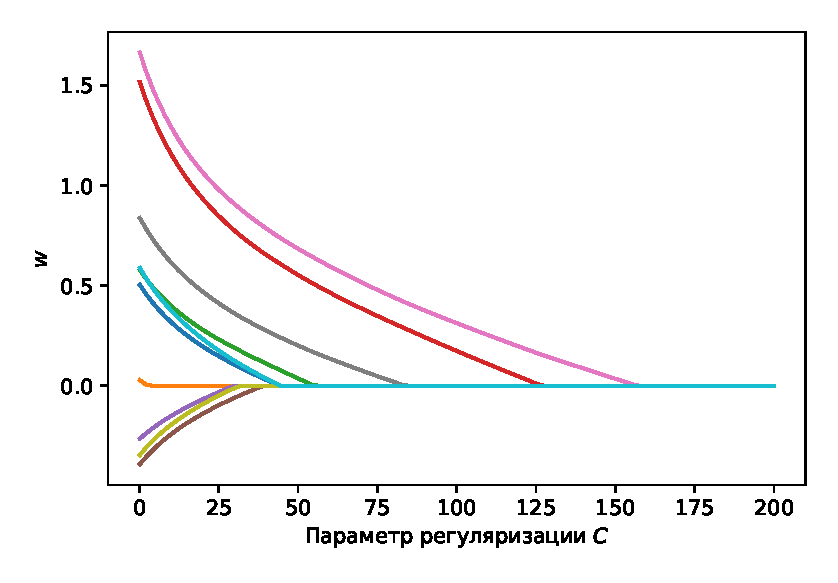
\includegraphics[width=0.5\textwidth]{../figures/log_reg_cs_exp.eps}
	\caption{Sample figure caption.}
	\label{fig:fig1}
\end{figure}

\subsection{Tables}
See awesome Table~\ref{tab:table}.

The documentation for \verb+booktabs+ (`Publication quality tables in LaTeX') is available from:
\begin{center}
	\url{https://www.ctan.org/pkg/booktabs}
\end{center}


\begin{table}
	\caption{Sample table title}
	\centering
	\begin{tabular}{lll}
		\toprule
		\multicolumn{2}{c}{Part}                   \\
		\cmidrule(r){1-2}
		Name     & Description     & Size ($\mu$m) \\
		\midrule
		Dendrite & Input terminal  & $\sim$100     \\
		Axon     & Output terminal & $\sim$10      \\
		Soma     & Cell body       & up to $10^6$  \\
		\bottomrule
	\end{tabular}
	\label{tab:table}
\end{table}

\subsection{Lists}
\begin{itemize}
	\item Lorem ipsum dolor sit amet
	\item consectetur adipiscing elit.
	\item Aliquam dignissim blandit est, in dictum tortor gravida eget. In ac rutrum magna.
\end{itemize}


\bibliographystyle{unsrtnat}
\bibliography{references}

\end{document}
